
%% bare_jrnl_compsoc.tex
%% V1.4b
%% 2015/08/26
%% by Michael Shell
%% See:
%% http://www.michaelshell.org/
%% for current contact information.
%%
%% This is a skeleton file demonstrating the use of IEEEtran.cls
%% (requires IEEEtran.cls version 1.8b or later) with an IEEE
%% Computer Society journal paper.
%%
%% Support sites:
%% http://www.michaelshell.org/tex/ieeetran/
%% http://www.ctan.org/pkg/ieeetran
%% and
%% http://www.ieee.org/

%%*************************************************************************
%% Legal Notice:
%% This code is offered as-is without any warranty either expressed or
%% implied; without even the implied warranty of MERCHANTABILITY or
%% FITNESS FOR A PARTICULAR PURPOSE! 
%% User assumes all risk.
%% In no event shall the IEEE or any contributor to this code be liable for
%% any damages or losses, including, but not limited to, incidental,
%% consequential, or any other damages, resulting from the use or misuse
%% of any information contained here.
%%
%% All comments are the opinions of their respective authors and are not
%% necessarily endorsed by the IEEE.
%%
%% This work is distributed under the LaTeX Project Public License (LPPL)
%% ( http://www.latex-project.org/ ) version 1.3, and may be freely used,
%% distributed and modified. A copy of the LPPL, version 1.3, is included
%% in the base LaTeX documentation of all distributions of LaTeX released
%% 2003/12/01 or later.
%% Retain all contribution notices and credits.
%% ** Modified files should be clearly indicated as such, including  **
%% ** renaming them and changing author support contact information. **
%%*************************************************************************


% *** Authors should verify (and, if needed, correct) their LaTeX system  ***
% *** with the testflow diagnostic prior to trusting their LaTeX platform ***
% *** with production work. The IEEE's font choices and paper sizes can   ***
% *** trigger bugs that do not appear when using other class files.       ***                          ***
% The testflow support page is at:
% http://www.michaelshell.org/tex/testflow/


\documentclass[10pt,journal,compsoc]{IEEEtran}
%
% If IEEEtran.cls has not been installed into the LaTeX system files,
% manually specify the path to it like:
% \documentclass[10pt,journal,compsoc]{../sty/IEEEtran}


% Some very useful LaTeX packages include:
% (uncomment the ones you want to load)


% *** MISC UTILITY PACKAGES ***
%
%\usepackage{ifpdf}
% Heiko Oberdiek's ifpdf.sty is very useful if you need conditional
% compilation based on whether the output is pdf or dvi.
% usage:
% \ifpdf
%   % pdf code
% \else
%   % dvi code
% \fi
% The latest version of ifpdf.sty can be obtained from:
% http://www.ctan.org/pkg/ifpdf
% Also, note that IEEEtran.cls V1.7 and later provides a builtin
% \ifCLASSINFOpdf conditional that works the same way.
% When switching from latex to pdflatex and vice-versa, the compiler may
% have to be run twice to clear warning/error messages.



\usepackage{listings}


% *** CITATION PACKAGES ***
%
\ifCLASSOPTIONcompsoc
  % IEEE Computer Society needs nocompress option
  % requires cite.sty v4.0 or later (November 2003)
  \usepackage[nocompress]{cite}
\else
  % normal IEEE
  \usepackage{cite}
\fi
% cite.sty was written by Donald Arseneau
% V1.6 and later of IEEEtran pre-defines the format of the cite.sty package
% \cite{} output to follow that of the IEEE. Loading the cite package will
% result in citation numbers being automatically sorted and properly
% "compressed/ranged". e.g., [1], [9], [2], [7], [5], [6] without using
% cite.sty will become [1], [2], [5]--[7], [9] using cite.sty. cite.sty's
% \cite will automatically add leading space, if needed. Use cite.sty's
% noadjust option (cite.sty V3.8 and later) if you want to turn this off
% such as if a citation ever needs to be enclosed in parenthesis.
% cite.sty is already installed on most LaTeX systems. Be sure and use
% version 5.0 (2009-03-20) and later if using hyperref.sty.
% The latest version can be obtained at:
% http://www.ctan.org/pkg/cite
% The documentation is contained in the cite.sty file itself.
%
% Note that some packages require special options to format as the Computer
% Society requires. In particular, Computer Society  papers do not use
% compressed citation ranges as is done in typical IEEE papers
% (e.g., [1]-[4]). Instead, they list every citation separately in order
% (e.g., [1], [2], [3], [4]). To get the latter we need to load the cite
% package with the nocompress option which is supported by cite.sty v4.0
% and later. Note also the use of a CLASSOPTION conditional provided by
% IEEEtran.cls V1.7 and later.





% *** GRAPHICS RELATED PACKAGES ***
%
\ifCLASSINFOpdf
  \usepackage{graphicx}
  % declare the path(s) where your graphic files are
  \graphicspath{{Figures/}{Other_Folder/}}
  % and their extensions so you won't have to specify these with
  % every instance of \includegraphics
  \DeclareGraphicsExtensions{.pdf,.jpeg,.png}
\else
  % or other class option (dvipsone, dvipdf, if not using dvips). graphicx
  % will default to the driver specified in the system graphics.cfg if no
  % driver is specified.
  % \usepackage[dvips]{graphicx}
  % declare the path(s) where your graphic files are
  % \graphicspath{{../eps/}}
  % and their extensions so you won't have to specify these with
  % every instance of \includegraphics
  % \DeclareGraphicsExtensions{.eps}
\fi
% graphicx was written by David Carlisle and Sebastian Rahtz. It is
% required if you want graphics, photos, etc. graphicx.sty is already
% installed on most LaTeX systems. The latest version and documentation
% can be obtained at: 
% http://www.ctan.org/pkg/graphicx
% Another good source of documentation is "Using Imported Graphics in
% LaTeX2e" by Keith Reckdahl which can be found at:
% http://www.ctan.org/pkg/epslatex
%
% latex, and pdflatex in dvi mode, support graphics in encapsulated
% postscript (.eps) format. pdflatex in pdf mode supports graphics
% in .pdf, .jpeg, .png and .mps (metapost) formats. Users should ensure
% that all non-photo figures use a vector format (.eps, .pdf, .mps) and
% not a bitmapped formats (.jpeg, .png). The IEEE frowns on bitmapped formats
% which can result in "jaggedy"/blurry rendering of lines and letters as
% well as large increases in file sizes.
%
% You can find documentation about the pdfTeX application at:
% http://www.tug.org/applications/pdftex






% *** MATH PACKAGES ***
%
%\usepackage{amsmath}
% A popular package from the American Mathematical Society that provides
% many useful and powerful commands for dealing with mathematics.
%
% Note that the amsmath package sets \interdisplaylinepenalty to 10000
% thus preventing page breaks from occurring within multiline equations. Use:
%\interdisplaylinepenalty=2500
% after loading amsmath to restore such page breaks as IEEEtran.cls normally
% does. amsmath.sty is already installed on most LaTeX systems. The latest
% version and documentation can be obtained at:
% http://www.ctan.org/pkg/amsmath





% *** SPECIALIZED LIST PACKAGES ***
%
%\usepackage{algorithmic}
% algorithmic.sty was written by Peter Williams and Rogerio Brito.
% This package provides an algorithmic environment fo describing algorithms.
% You can use the algorithmic environment in-text or within a figure
% environment to provide for a floating algorithm. Do NOT use the algorithm
% floating environment provided by algorithm.sty (by the same authors) or
% algorithm2e.sty (by Christophe Fiorio) as the IEEE does not use dedicated
% algorithm float types and packages that provide these will not provide
% correct IEEE style captions. The latest version and documentation of
% algorithmic.sty can be obtained at:
% http://www.ctan.org/pkg/algorithms
% Also of interest may be the (relatively newer and more customizable)
% algorithmicx.sty package by Szasz Janos:
% http://www.ctan.org/pkg/algorithmicx




% *** ALIGNMENT PACKAGES ***
%
%\usepackage{array}
% Frank Mittelbach's and David Carlisle's array.sty patches and improves
% the standard LaTeX2e array and tabular environments to provide better
% appearance and additional user controls. As the default LaTeX2e table
% generation code is lacking to the point of almost being broken with
% respect to the quality of the end results, all users are strongly
% advised to use an enhanced (at the very least that provided by array.sty)
% set of table tools. array.sty is already installed on most systems. The
% latest version and documentation can be obtained at:
% http://www.ctan.org/pkg/array


% IEEEtran contains the IEEEeqnarray family of commands that can be used to
% generate multiline equations as well as matrices, tables, etc., of high
% quality.




% *** SUBFIGURE PACKAGES ***
\ifCLASSOPTIONcompsoc
 \usepackage[caption=false,font=footnotesize,labelfont=sf,textfont=sf]{subfig}
\else
 \usepackage[caption=false,font=footnotesize]{subfig}
\fi
% subfig.sty, written by Steven Douglas Cochran, is the modern replacement
% for subfigure.sty, the latter of which is no longer maintained and is
% incompatible with some LaTeX packages including fixltx2e. However,
% subfig.sty requires and automatically loads Axel Sommerfeldt's caption.sty
% which will override IEEEtran.cls' handling of captions and this will result
% in non-IEEE style figure/table captions. To prevent this problem, be sure
% and invoke subfig.sty's "caption=false" package option (available since
% subfig.sty version 1.3, 2005/06/28) as this is will preserve IEEEtran.cls
% handling of captions.
% Note that the Computer Society format requires a sans serif font rather
% than the serif font used in traditional IEEE formatting and thus the need
% to invoke different subfig.sty package options depending on whether
% compsoc mode has been enabled.
%
% The latest version and documentation of subfig.sty can be obtained at:
% http://www.ctan.org/pkg/subfig



% *** FLOAT PACKAGES ***
%
%\usepackage{fixltx2e}
% fixltx2e, the successor to the earlier fix2col.sty, was written by
% Frank Mittelbach and David Carlisle. This package corrects a few problems
% in the LaTeX2e kernel, the most notable of which is that in current
% LaTeX2e releases, the ordering of single and double column floats is not
% guaranteed to be preserved. Thus, an unpatched LaTeX2e can allow a
% single column figure to be placed prior to an earlier double column
% figure.
% Be aware that LaTeX2e kernels dated 2015 and later have fixltx2e.sty's
% corrections already built into the system in which case a warning will
% be issued if an attempt is made to load fixltx2e.sty as it is no longer
% needed.
% The latest version and documentation can be found at:
% http://www.ctan.org/pkg/fixltx2e


%\usepackage{stfloats}
% stfloats.sty was written by Sigitas Tolusis. This package gives LaTeX2e
% the ability to do double column floats at the bottom of the page as well
% as the top. (e.g., "\begin{figure*}[!b]" is not normally possible in
% LaTeX2e). It also provides a command:
%\fnbelowfloat
% to enable the placement of footnotes below bottom floats (the standard
% LaTeX2e kernel puts them above bottom floats). This is an invasive package
% which rewrites many portions of the LaTeX2e float routines. It may not work
% with other packages that modify the LaTeX2e float routines. The latest
% version and documentation can be obtained at:
% http://www.ctan.org/pkg/stfloats
% Do not use the stfloats baselinefloat ability as the IEEE does not allow
% \baselineskip to stretch. Authors submitting work to the IEEE should note
% that the IEEE rarely uses double column equations and that authors should try
% to avoid such use. Do not be tempted to use the cuted.sty or midfloat.sty
% packages (also by Sigitas Tolusis) as the IEEE does not format its papers in
% such ways.
% Do not attempt to use stfloats with fixltx2e as they are incompatible.
% Instead, use Morten Hogholm'a dblfloatfix which combines the features
% of both fixltx2e and stfloats:
%
% \usepackage{dblfloatfix}
% The latest version can be found at:
% http://www.ctan.org/pkg/dblfloatfix




%\ifCLASSOPTIONcaptionsoff
%  \usepackage[nomarkers]{endfloat}
% \let\MYoriglatexcaption\caption
% \renewcommand{\caption}[2][\relax]{\MYoriglatexcaption[#2]{#2}}
%\fi
% endfloat.sty was written by James Darrell McCauley, Jeff Goldberg and 
% Axel Sommerfeldt. This package may be useful when used in conjunction with 
% IEEEtran.cls'  captionsoff option. Some IEEE journals/societies require that
% submissions have lists of figures/tables at the end of the paper and that
% figures/tables without any captions are placed on a page by themselves at
% the end of the document. If needed, the draftcls IEEEtran class option or
% \CLASSINPUTbaselinestretch interface can be used to increase the line
% spacing as well. Be sure and use the nomarkers option of endfloat to
% prevent endfloat from "marking" where the figures would have been placed
% in the text. The two hack lines of code above are a slight modification of
% that suggested by in the endfloat docs (section 8.4.1) to ensure that
% the full captions always appear in the list of figures/tables - even if
% the user used the short optional argument of \caption[]{}.
% IEEE papers do not typically make use of \caption[]'s optional argument,
% so this should not be an issue. A similar trick can be used to disable
% captions of packages such as subfig.sty that lack options to turn off
% the subcaptions:
% For subfig.sty:
% \let\MYorigsubfloat\subfloat
% \renewcommand{\subfloat}[2][\relax]{\MYorigsubfloat[]{#2}}
% However, the above trick will not work if both optional arguments of
% the \subfloat command are used. Furthermore, there needs to be a
% description of each subfigure *somewhere* and endfloat does not add
% subfigure captions to its list of figures. Thus, the best approach is to
% avoid the use of subfigure captions (many IEEE journals avoid them anyway)
% and instead reference/explain all the subfigures within the main caption.
% The latest version of endfloat.sty and its documentation can obtained at:
% http://www.ctan.org/pkg/endfloat
%
% The IEEEtran \ifCLASSOPTIONcaptionsoff conditional can also be used
% later in the document, say, to conditionally put the References on a 
% page by themselves.




% *** PDF, URL AND HYPERLINK PACKAGES ***
%
\usepackage{url}
\usepackage{hyperref}
% url.sty was written by Donald Arseneau. It provides better support for
% handling and breaking URLs. url.sty is already installed on most LaTeX
% systems. The latest version and documentation can be obtained at:
% http://www.ctan.org/pkg/url
% Basically, \url{my_url_here}.





% *** Do not adjust lengths that control margins, column widths, etc. ***
% *** Do not use packages that alter fonts (such as pslatex).         ***
% There should be no need to do such things with IEEEtran.cls V1.6 and later.
% (Unless specifically asked to do so by the journal or conference you plan
% to submit to, of course. )


% correct bad hyphenation here
\hyphenation{op-tical net-works semi-conduc-tor}


\usepackage{xcolor}
% Define a style for syntax highlighting
\lstdefinestyle{mystyle}{
    basicstyle=\small\ttfamily,
    keywordstyle=\color{blue},
    commentstyle=\color{green!50!black},
    stringstyle=\color{black!25!green},
    breaklines=true,
    frame=single,
    rulecolor=\color{black!30},
    backgroundcolor=\color{gray!5},
    morekeywords={func_4_1, update, additionalWord1, additionalWord2, __global__},
    keywordstyle={[2]\color{purple}}, % additionalWord1
    keywordstyle={[3]\color{orange}}, % additionalWord2
    keywordstyle={[4]\color{red}}, % __global__
}
\usepackage{float}
\usepackage{graphicx}
%\usepackage{caption}
\usepackage{multicol,caption}
\usepackage{graphicx}
%\usepackage{lipsum}
%\newenvironment{Figure}
%  {\par\medskip\noindent\minipage{\linewidth}}
%  {\endminipage\par\medskip}
\usepackage{url}
\usepackage{hyperref}

\begin{document}


%
% paper title
% Titles are generally capitalized except for words such as a, an, and, as,
% at, but, by, for, in, nor, of, on, or, the, to and up, which are usually
% not capitalized unless they are the first or last word of the title.
% Linebreaks \\ can be used within to get better formatting as desired.
% Do not put math or special symbols in the title.
\title{Storms of High-energy Particles}
%
%
% author names and IEEE memberships
% note positions of commas and nonbreaking spaces ( ~ ) LaTeX will not break
% a structure at a ~ so this keeps an author's name from being broken across
% two lines.
% use \thanks{} to gain access to the first footnote area
% a separate \thanks must be used for each paragraph as LaTeX2e's \thanks
% was not built to handle multiple paragraphs
%
%
%\IEEEcompsocitemizethanks is a special \thanks that produces the bulleted
% lists the Computer Society journals use for "first footnote" author
% affiliations. Use \IEEEcompsocthanksitem which works much like \item
% for each affiliation group. When not in compsoc mode,
% \IEEEcompsocitemizethanks becomes like \thanks and
% \IEEEcompsocthanksitem becomes a line break with idention. This
% facilitates dual compilation, although admittedly the differences in the
% desired content of \author between the different types of papers makes a
% one-size-fits-all approach a daunting prospect. For instance, compsoc 
% journal papers have the author affiliations above the "Manuscript
% received ..."  text while in non-compsoc journals this is reversed. Sigh.

\author{João~Tomás and %~\IEEEmembership{Member,~IEEE,}%
        Renato~Viola, \IEEEmembership{Universidade Nova De Lisboa,~Faculdade de Ciências e Tecnologia}%
        %and~Jane~Doe,~\IEEEmembership{Life~Fellow,~IEEE}% <-this % stops a space
\IEEEcompsocitemizethanks{\IEEEcompsocthanksitem João~Tomás and Renato~Viola are with the Department
of Computer Engineering, Universidade Nova de Lisboa, Faculdade de Ciencias e Tecnologia.\protect\\
% note need leading \protect in front of \\ to get a newline within \thanks as
% \\ is fragile and will error, could use \hfil\break instead.
E-mail: jl.tomas@campus.fct.unl.pt
E-mail: r.viola@campus.fct.unl.pt
\IEEEcompsocthanksitem J.Tomás and R.Viola are with FCT UNL.}% <-this % stops an unwanted space
\thanks{}}

% note the % following the last \IEEEmembership and also \thanks - 
% these prevent an unwanted space from occurring between the last author name
% and the end of the author line. i.e., if you had this:
% 
% \author{....lastname \thanks{...} \thanks{...} }
%                     ^------------^------------^----Do not want these spaces!
%
% a space would be appended to the last name and could cause every name on that
% line to be shifted left slightly. This is one of those "LaTeX things". For
% instance, "\textbf{A} \textbf{B}" will typeset as "A B" not "AB". To get
% "AB" then you have to do: "\textbf{A}\textbf{B}"
% \thanks is no different in this regard, so shield the last } of each \thanks
% that ends a line with a % and do not let a space in before the next \thanks.
% Spaces after \IEEEmembership other than the last one are OK (and needed) as
% you are supposed to have spaces between the names. For what it is worth,
% this is a minor point as most people would not even notice if the said evil
% space somehow managed to creep in.



% The paper headers
\markboth{CAD REPORT}%
{Shell \MakeLowercase{\textit{et al.}}: Bare Demo of IEEEtran.cls for Computer Society Journals}
% The only time the second header will appear is for the odd numbered pages
% after the title page when using the twoside option.
% 
% *** Note that you probably will NOT want to include the author's ***
% *** name in the headers of peer review papers.                   ***
% You can use \ifCLASSOPTIONpeerreview for conditional compilation here if
% you desire.



% The publisher's ID mark at the bottom of the page is less important with
% Computer Society journal papers as those publications place the marks
% outside of the main text columns and, therefore, unlike regular IEEE
% journals, the available text space is not reduced by their presence.
% If you want to put a publisher's ID mark on the page you can do it like
% this:
%\IEEEpubid{0000--0000/00\$00.00~\copyright~2015 IEEE}
% or like this to get the Computer Society new two part style.
%\IEEEpubid{\makebox[\columnwidth]{\hfill 0000--0000/00/\$00.00~\copyright~2015 IEEE}%
%\hspace{\columnsep}\makebox[\columnwidth]{Published by the IEEE Computer Society\hfill}}
% Remember, if you use this you must call \IEEEpubidadjcol in the second
% column for its text to clear the IEEEpubid mark (Computer Society jorunal
% papers don't need this extra clearance.)



% use for special paper notices
%\IEEEspecialpapernotice{(Invited Paper)}



% for Computer Society papers, we must declare the abstract and index terms
% PRIOR to the title within the \IEEEtitleabstractindextext IEEEtran
% command as these need to go into the title area created by \maketitle.
% As a general rule, do not put math, special symbols or citations
% in the abstract or keywords.

%Idea we had a code that did a simulation and we used cuda try to improve it, the first thing we did was the refactoring of the code we divided it into functions so that we then could use a profiler to see where bottlenecks were present after this we began our CUDA implementation %
\IEEEtitleabstractindextext{%
\begin{abstract}
In this paper we will explore how beneficial a CUDA implementation on a sequential program can be. Utilizing tools for code analysis, we aim to gain a comprehensive understanding of the specific areas where our program experiences slowdowns. Throughout this paper we will show charts of the first and final results, examples of changes that were made in the original code and our final view on this work.

\end{abstract}

% Note that keywords are not normally used for peerreview papers.
\begin{IEEEkeywords}
Computer Science, Profiling, CUDA.
\end{IEEEkeywords}}


% make the title area
\maketitle


% To allow for easy dual compilation without having to reenter the
% abstract/keywords data, the \IEEEtitleabstractindextext text will
% not be used in maketitle, but will appear (i.e., to be "transported")
% here as \IEEEdisplaynontitleabstractindextext when the compsoc 
% or transmag modes are not selected <OR> if conference mode is selected 
% - because all conference papers position the abstract like regular
% papers do.
\IEEEdisplaynontitleabstractindextext
% \IEEEdisplaynontitleabstractindextext has no effect when using
% compsoc or transmag under a non-conference mode.



% For peer review papers, you can put extra information on the cover
% page as needed:
% \ifCLASSOPTIONpeerreview
% \begin{center} \bfseries EDICS Category: 3-BBND \end{center}
% \fi
%
% For peerreview papers, this IEEEtran command inserts a page break and
% creates the second title. It will be ignored for other modes.
\IEEEpeerreviewmaketitle



\IEEEraisesectionheading{\section{Introduction}\label{sec:introduction}}
% Computer Society journal (but not conference!) papers do something unusual
% with the very first section heading (almost always called "Introduction").
% They place it ABOVE the main text! IEEEtran.cls does not automatically do
% this for you, but you can achieve this effect with the provided
% \IEEEraisesectionheading{} command. Note the need to keep any \label that
% is to refer to the section immediately after \section in the above as
% \IEEEraisesectionheading puts \section within a raised box.




% The very first letter is a 2 line initial drop letter followed
% by the rest of the first word in caps (small caps for compsoc).
% 
% form to use if the first word consists of a single letter:
% \IEEEPARstart{A}{demo} file is ....
% 
% form to use if you need the single drop letter followed by
% normal text (unknown if ever used by the IEEE):
% \IEEEPARstart{A}{}demo file is ....
% 
% Some journals put the first two words in caps:
% \IEEEPARstart{T}{his demo} file is ....
% 
% Here we have the typical use of a "T" for an initial drop letter
% and "HIS" in caps to complete the first word.
\IEEEPARstart{I}{n} this paper, we will be tackling the parallelization of a sequential program simulating the effects of the bombardment of an exposed surface with waves of high-energy particles. \par
To our convenience, the provided program presents us this problem in a simplified manner by considering only a cross-section of the surface, represented by equally distributed control points on the outermost layer of the material. However, as expected from any problem involving particles, we can potentially be dealing with very large sets of data. \par
In this particular case, we must take into account not only the great number of particles that may be present, but also the number of control points, which could very well be in the tens or even hundreds of millions. In a realistic scenario, these operations can become quite resource-intensive and computationally demanding, hindering scalability and execution time in significant ways. \par
We aim to optimize this program and substantially improve its execution speed by harnessing the power of parallel processing in GPUs, whilst maintaining the very same functionality and correctness of the provided sequential code. To this end, we will be integrating CUDA in our approach. \par
We began by analysing the code to break it down for factorization, allowing us to subsequently employ profiling tools. This approach enabled us to pinpoint a good starting point for our CUDA optimizations.
% You must have at least 2 lines in the paragraph with the drop letter
% (should never be an issue)



 
\hfill November 12, 2023

%\subsection{Subsection Heading Here}
%Subsection text here.

% needed in second column of first page if using \IEEEpubid
%\IEEEpubidadjcol

%\subsubsection{Subsubsection Heading Here}
%Subsubsection text here.


% An example of a floating figure using the graphicx package.
% Note that \label must occur AFTER (or within) \caption.
% For figures, \caption should occur after the \includegraphics.
% Note that IEEEtran v1.7 and later has special internal code that
% is designed to preserve the operation of \label within \caption
% even when the captionsoff option is in effect. However, because
% of issues like this, it may be the safest practice to put all your
% \label just after \caption rather than within \caption{}.
%
% Reminder: the "draftcls" or "draftclsnofoot", not "draft", class
% option should be used if it is desired that the figures are to be
% displayed while in draft mode.
%
%\begin{figure}[!t]
%\centering
%\includegraphics[width=2.5in]{myfigure}
% where an .eps filename suffix will be assumed under latex, 
% and a .pdf suffix will be assumed for pdflatex; or what has been declared
% via \DeclareGraphicsExtensions.
%\caption{Simulation results for the network.}
%\label{fig_sim}
%\end{figure}

% Note that the IEEE typically puts floats only at the top, even when this
% results in a large percentage of a column being occupied by floats.
% However, the Computer Society has been known to put floats at the bottom.


% An example of a double column floating figure using two subfigures.
% (The subfig.sty package must be loaded for this to work.)
% The subfigure \label commands are set within each subfloat command,
% and the \label for the overall figure must come after \caption.
% \hfil is used as a separator to get equal spacing.
% Watch out that the combined width of all the subfigures on a 
% line do not exceed the text width or a line break will occur.
%
%\begin{figure*}[!t]
%\centering
%\subfloat[Case I]{\includegraphics[width=2.5in]{box}%
%\label{fig_first_case}}
%\hfil
%\subfloat[Case II]{\includegraphics[width=2.5in]{box}%
%\label{fig_second_case}}
%\caption{Simulation results for the network.}
%\label{fig_sim}
%\end{figure*}
%
% Note that often IEEE papers with subfigures do not employ subfigure
% captions (using the optional argument to \subfloat[]), but instead will
% reference/describe all of them (a), (b), etc., within the main caption.
% Be aware that for subfig.sty to generate the (a), (b), etc., subfigure
% labels, the optional argument to \subfloat must be present. If a
% subcaption is not desired, just leave its contents blank,
% e.g., \subfloat[].


% An example of a floating table. Note that, for IEEE style tables, the
% \caption command should come BEFORE the table and, given that table
% captions serve much like titles, are usually capitalized except for words
% such as a, an, and, as, at, but, by, for, in, nor, of, on, or, the, to
% and up, which are usually not capitalized unless they are the first or
% last word of the caption. Table text will default to \footnotesize as
% the IEEE normally uses this smaller font for tables.
% The \label must come after \caption as always.
%
%\begin{table}[!t]
%% increase table row spacing, adjust to taste
%\renewcommand{\arraystretch}{1.3}
% if using array.sty, it might be a good idea to tweak the value of
% \extrarowheight as needed to properly center the text within the cells
%\caption{An Example of a Table}
%\label{table_example}
%\centering
%% Some packages, such as MDW tools, offer better commands for making tables
%% than the plain LaTeX2e tabular which is used here.
%\begin{tabular}{|c||c|}
%\hline
%One & Two\\
%\hline
%Three & Four\\
%\hline
%\end{tabular}
%\end{table}


% Note that the IEEE does not put floats in the very first column
% - or typically anywhere on the first page for that matter. Also,
% in-text middle ("here") positioning is typically not used, but it
% is allowed and encouraged for Computer Society conferences (but
% not Computer Society journals). Most IEEE journals/conferences use
% top floats exclusively. 
% Note that, LaTeX2e, unlike IEEE journals/conferences, places
% footnotes above bottom floats. This can be corrected via the
% \fnbelowfloat command of the stfloats package.

\section{Methodology}

\subsection{Code Factorization }
After an initial analysis of the code, we had a decent understanding of its structure and functionality. Following this, we reorganized some of the code into well-defined functions, named after the section their respective code was in, in order to facilitate the profiling that would take place later on.

\subsection{Profiling \& CUDA implementation}
With the code refactored and modularized, we can now make effective use of profilers to help us identify performance bottlenecks within the code.
Instead of proceeding blindly and attempting to simply parallelize everything right away, we used 
\textit{gprof} to help us decide where to prioritize our efforts - probably where the optimizations could yield the most significant improvements. For the parallelized version of the code, we utilized NVIDIA's own profiler for CUDA applications, \textit{nvprof}, which provided us with a detailed breakdown of GPU kernel executions alongside other GPU-specific metrics.

In the following Pie charts we can see the percentages of time that each function was taking in the sequential version of the code with gprof, on tests 2, 7 and 8 with 30.000, 1.000.000 and 100.000.000 control points, respectively.
\begin{figure}[H]
 \centering
 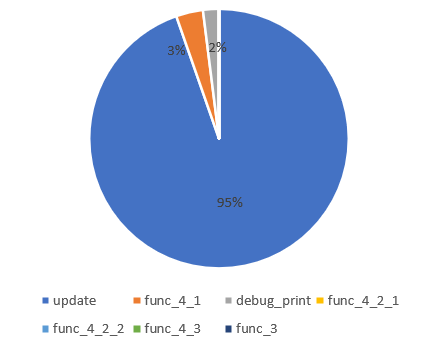
\includegraphics[width=0.8\linewidth]{img/gprof_2_30000.png}
 \captionof{figure}{Sequential Test 2 positions=30000}
\end{figure}

\onecolumn
\begin{multicols}{2}
\begin{figure}[H]
 \centering
 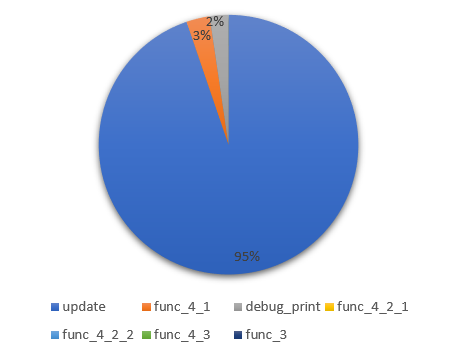
\includegraphics[width=0.8\linewidth]{img/gprof_7_1000000.png}
 \captionof{figure}{Sequential Test 7 positions=1000000}
\end{figure}

%\newline
\begin{figure}[H]
 \centering
 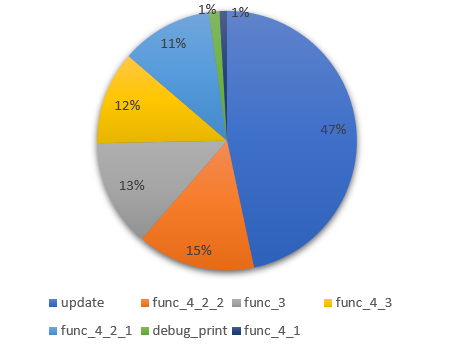
\includegraphics[width=0.8\linewidth]{img/gprof_8_100000000.png}
 \captionof{figure}{Sequential Test 8 positions=100000000}
\end{figure}
\end{multicols}


From now on our focus moves to the parallelization of the more intense tasks that we were able to catch with the profiler. Following each optimization, we conduct tests and compare the results with the sequential version to assess the impact of the change on our program


\section{Code Analysis \& Examples}

\par From the profiling on tests 2 and 7, we have detected that a large portion of the running time is due to the 'update' method being called many times. So this was our primary focus at this point.

As previously stated, \texttt{update} is being called a great number of times, so optimizing this function itself would be a step in the right direction. However, we weren't really sure how to optimize this method's logic without breaking it, so we left it as is.
Our alternative was to optimize the function that calls \texttt{update} all these times, which is \texttt{func\-\_4\-\_1}.

\begin{lstlisting}[
    style=mystyle,
    language=C,
    caption=Sequential code,
    basicstyle=\ttfamily,
    breaklines=true,
    breakatwhitespace=true,
    linewidth=\textwidth
]
 void func_4_1(int i, Storm storms[], int layer_size, float *layer) {
    for (int j = 0; j < storms[i].size; j++) {
        float energy = (float)storms[i].posval[j * 2 + 1] * 1000;
        int position = storms[i].posval[j * 2];
        for (int k = 0; k < layer_size; k++) {
            update(layer, layer_size, k, position, energy);
        }
    }
}
\end{lstlisting}
We paralellized it by translating the function's most inner loop into a CUDA kernel: 
\begin{itemize}
  \item A thread is identified by its thread and block indices, as well as block dimension.
  \item We ensure that the thread is operating within the bounds of the layer with a conditional check.
  \item Each thread computes the \texttt{update} operation independently for a different cell.
\end{itemize}


\begin{lstlisting}[
    style=mystyle,
    language=C,
    caption=CUDA code,
    basicstyle=\ttfamily,
    breaklines=true,
    breakatwhitespace=true,
    linewidth=\textwidth
]
 __global__ void func_4_1(int layer_size, float *d_layer, int position, float energy) {
    int index = blockIdx.x * blockDim.x + threadIdx.x;
    if (index < layer_size)
        update(d_layer, layer_size, index, position, energy);
}

\end{lstlisting}

After making this change, we noticed a very significant performance boost in the time our code took to run tests 2 and 7,
with the control point values mentioned above.

We then moved on to the optimization of \texttt{func\-\_4\-\_2\-\_2}, which was also shown to be somewhat of a hotspot.

\begin{lstlisting}[
    style=mystyle,
    language=C,
    caption=Sequential code,
    basicstyle=\ttfamily,
    breaklines=true,
    breakatwhitespace=true,
    linewidth=\textwidth
]
void func_4_2_2(int layer_size, float *layer, float *layer_copy) {
    for (int k = 1; k < layer_size - 1; k++)
        layer[k] = (layer_copy[k - 1] + layer_copy[k] + layer_copy[k + 1]) / 3;
}

\end{lstlisting}


In this method, each element in the \texttt{layer} array is updated based on its own value and also the values of its adjacent
neighbors in the \texttt{layer\_copy} array, a stencil operation. Using shared memory here would have proved most useful, but at the time we hadn't researched the subject enough to implement it correctly. We approached this method very similarly to how we did for \texttt{func\_4\_1}, although with slight changes to the conditional check. Due to time constraints, we couldn't revisit this function and implement the shared memory approach.


\begin{lstlisting}[
    style=mystyle,
    language=C,
    caption=CUDA code,
    basicstyle=\ttfamily,
    breaklines=true,
    breakatwhitespace=true,
    linewidth=\textwidth
]
__global__ void func_4_2_2(int layer_size, float *d_layer, float *d_layer_copy) {
    int index = blockIdx.x * blockDim.x + threadIdx.x;
    if (index > 0 && index < layer_size - 1)
        d_layer[index] = (d_layer_copy[index - 1] + d_layer_copy[index] + d_layer_copy[index + 1]) / 3;
}
\end{lstlisting}

Aside from \texttt{func\-\_4\-\_3}, the remaining functions, \texttt{func\-\_3} and \texttt{func\-\_4\-\_2\-\_1}, were parallelized much in the same manner as \texttt{func\-\_4\-\_1}, varying only in the actual operation they execute.

The profiler of test 8 indicates that, \texttt{func\-\_4\-\_3} is the one taking the most time to execute.
Unlike the other functions this one was not so direct, a naive implementation could lead to data races. Not only does the computation of each element depend on its neighboring elements, but also the innermost if-statement compares an element to the current known global maximum after asserting that it was a local maximum. 

\begin{minipage}{\linewidth}
\begin{lstlisting}[
    style=mystyle,
    language=C,
    caption=CUDA code,
    basicstyle=\ttfamily,
    breaklines=true,
    breakatwhitespace=true,
    linewidth=\textwidth
]
void func_4_3(int i, int layer_size, float *layer, float maximum[], int positions[])
{
    for (int k = 1; k < layer_size - 1; k++) {
        if (layer[k] > layer[k - 1] && layer[k] > layer[k + 1]) {
            if (layer[k] > maximum[i]) {
                maximum[i] = layer[k];
                positions[i] = k;
            }
        }
    }
}
\end{lstlisting}
\end{minipage}
\par The problem required some sort of synchronization, as we need to ensure all local maxima are being considered before we can effectively calculate the global maximum and its position. Our solution was to use a parallel reduction in order to find the local maximum for each block, and perform a final, much smaller reduction on the CPU to find the global maximum across all blocks.
We chose Sequential Addressing over Interleaved Addressing as the strategy for our reduction, as it is bank conflict free and no more difficult to implement. To do this we got ideas from this \cite{CudaSlides} slides, the \cite{Reduction} github code and also from this youtube video \cite{ReductionVideo}.

\begin{itemize}
  \item \texttt{sdata} and \texttt{sindices} are shared memory arrays which are used to store the values and indices of potential maxima found within the block;
  \item Each thread within the bounds of the layer loads an element from \texttt{d\-\_layer\-\_3} and its corresponding index into the shared memory structures;
  \item A loop iteratively checks for local maxima within the range of elements in shared memory, where each thread within the valid range of comparison compares elements separated by the stride distance and keeps the maximum value, as well as its index.
  \item The first thread in each block will write the block's maximum value and index in the global memory's arrays.
  \item Having every block's maximum, a final reduction is performed in the CPU to find the overall maximum and its position, which are then stored in \texttt{maximum[i]} and \texttt{positions[i]}.
\end{itemize}

\begin{minipage}{\linewidth}
\begin{lstlisting}[
    style=mystyle,
    language=C,
    caption=CUDA code,
    basicstyle=\ttfamily,
    breaklines=true,
    breakatwhitespace=true,
    linewidth=\textwidth
]
__global__ void func_4_3_kernel(float *d_layer, float *d_maxValues, int *d_maxPositions, int layer_size) {
    
    __shared__ float sdata[THREADS_PER_BLOCK];
    __shared__ int sindices[THREADS_PER_BLOCK];

    int tid = threadIdx.x;
    int idx = blockIdx.x * blockDim.x + threadIdx.x;

    if (idx < layer_size) {
        sdata[tid] = d_layer[idx];
        sindices[tid] = idx;
    }
    __syncthreads();
    for (unsigned int s = THREADS_PER_BLOCK / 2; s > 0; s /= 2) {
        int strideIndex = tid + s;
        if (tid < s && strideIndex < layer_size - 1) {
            if (sdata[strideIndex] > sdata[strideIndex - 1] && sdata[strideIndex] > sdata[strideIndex + 1]) {
                if (sdata[tid] < sdata[strideIndex]) {
                    sdata[tid] = sdata[strideIndex];
                    sindices[tid] = sindices[strideIndex];
                }
            }
        }
        __syncthreads();
    }
    if (tid == 0) {
        d_maxValues[blockIdx.x] = sdata[0];
        d_maxPositions[blockIdx.x] = sindices[0];
    }
}
\end{lstlisting}
\end{minipage}

\begin{minipage}{\linewidth}
\begin{lstlisting}[
    style=mystyle,
    language=C,
    caption=CUDA code,
    basicstyle=\ttfamily,
    breaklines=true,
    breakatwhitespace=true,
    linewidth=\textwidth
]
void func_4_3(int i, int layer_size, int nBlocks, float *d_layer, float *maximum, int *positions) {
    //MEMORY ALLOCATING

    func_4_3_kernel<<<nBlocks, THREADS_PER_BLOCK>>>
                (d_layer, d_maxValues, d_maxPositions, layer_size);
    
    //CUDA MEMCPY

    float max = -MAXFLOAT;
    int pos = -1;

    for (int j = 0; j < nBlocks; j++) {
        if (maxValues[j] > max) {
            max = maxValues[j];
            pos = maxPositions[j];
        }
    }

    maximum[i] = max;
    positions[i] = pos;
    //CUDA FREE...
}
\end{lstlisting}
\end{minipage}


\begin{multicols}{2}
\section{Results}
\subsection{Final Profilers}
%Data last profilers

%TODO
\begin{figure}[H]
 \centering
 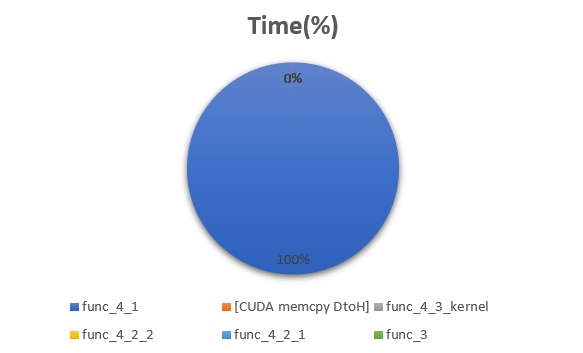
\includegraphics[width=\linewidth]{img/nvprof_2_30000.png}
 \captionof{figure}{CUDA Test 2 positions=30000}
\end{figure}
In this Pie chart we can see that the function where the program is taking the most time is the  \texttt{func\-\_4\-\_1} with percentage close to 100\%.

\begin{figure}[H]
 \centering
 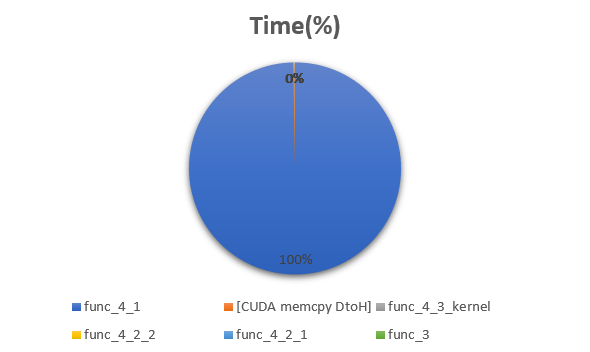
\includegraphics[width=\linewidth]{img/nvprof_7_1000000.png}
 \captionof{figure}{CUDA Test 7 positions=1000000}
\end{figure}

\begin{figure}[H]
 \centering
 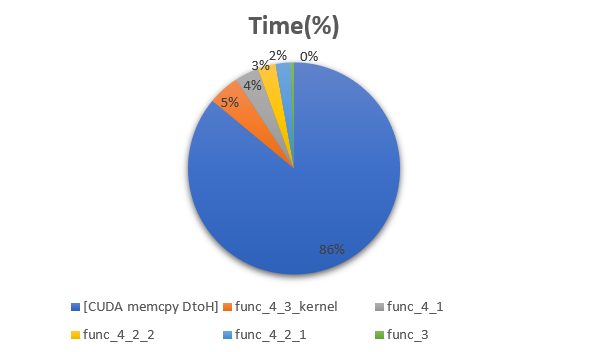
\includegraphics[width=\linewidth]{img/nvprof_8_100000000.png}
 \captionof{figure}{CUDA Test 8 positions=100000000}
 \end{figure}

In this last chart the percentages of each function get more spread, in this case the \texttt{func\-\_4\-\_1} is not the highest percentage and instead we get the \texttt{memcpy}, this shift can be attributed to the specific elements being tested under the conditions of test 8.

%\subsection{Paralellization}
%Data from the second profiler and execution time for the same inputs of above.

\subsection{Test Machine}
GPU:
\begin{lstlisting}[
    style=mystyle,
    language=C,
    basicstyle=\scriptsize\ttfamily,
    breaklines=true,
    breakatwhitespace=true,
    linewidth=\textwidth
]
Device 0: "NVIDIA GeForce GTX 1650 Ti"
  CUDA Driver Version / Runtime Version        12.2 / 11.5
  CUDA Capability Major/Minor version number:  7.5
  16 Multiprocessors (SM)
  Max Grid sizes: 2147483647, 65535, 65535
  Max Block sizes: 1024, 1024, 64
  Max Blocks per SM: 16
  Max threads per Block: 1024, Warp size: 32
  Total global memory: 4193984 MB
  Shared Mem per SM: 65536, Max ShMem per Block: 49152
\end{lstlisting}
CPU: AMD Ryzen 5 4600H\newline
RAM: 8GB


\subsection{Final Results}
\begin{figure}[H]
 \centering
 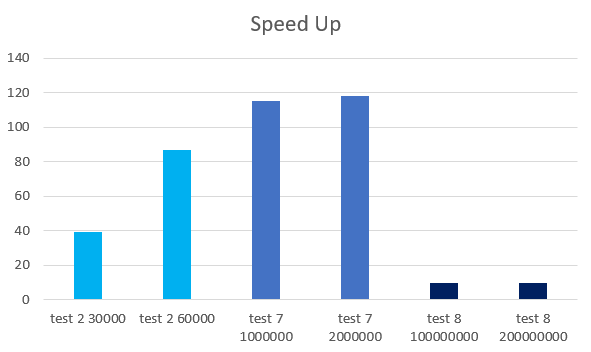
\includegraphics[width=\linewidth]{img/speedupBars.png}
 \captionof{figure}{Speed Up for Tests 2, 7 and 8}
\end{figure}

Here we have a chart that represents the final speed up of the different tests with two different inputs. The Y represents the speed up of the parallel version comparatively at the sequential one.


\section{Group Working Methodology}
During this project we used the ”Visual Studio Code” text editor in which we occasionally coded simultaneously by using the extension ”Live Share”. Most of the time though, we split tasks between us and worked individually, while maintaining contact to stay informed about each other's progress. For example, while one of us was working on the script, the other would be handling the report or profiling the code. The report was mostly a joint effort of both of us. Overall, we believe we distributed the workload evenly and that our work complemented each other's, achieving a 50/50 split. 

\section{Acknowledgments}
We would like to thank our colleagues Nelson Matos (60483) and Pedro Estróia (60691), who indicated us to Max Kotlan's
Github repository where there are several implementations of maximum-value algorithms, using the parallel reduction pattern.
The reduction pattern was the most challenging section of the project by far and it wasn't very easy to find references to anything other than sum reductions.
It would have taken us a lot longer to implement this pattern, had it not been for this reference, which was basically our guideline.

We'd also like to thank our professors for their availability to help.

\section{Comments, criticisms, and suggestions}
This was a very pleasant and interesting project to have worked on.
Its theme itself was already captivating, and in terms of difficulty we found it quite well-balanced.
It was challenging in some parts, while not being exhaustive. Not all optimizations could be approached 
the same way, some were varied and we were given the freedom to explore different ways to tackle them.
As we had to push ourselves to properly learn and adapt concepts to our program, we grew more comfortable with 
parallel programming in general.


\section{Conclusion}
We started this project with the idea of getting a sequential program to have better performance by parallelizing it using a CUDA implementation. Throughout this paper we were able to show that our program did in fact run faster as shown in the results section. The recommended methodology that focused on the repeating steps of using a profiler to find the hot-spots/bottlenecks and then parallelizing, proved to be a highly effective strategy as we could shift our focus on was more important. %"as we were always getting better results".
Though we acknowledge that our solution has some room for improvement, we are very pleased with the results we have obtained
and what we've learned as well.



% if have a single appendix:
%\appendix[Proof of the Zonklar Equations]
% or
%\appendix  % for no appendix heading
% do not use \section anymore after \appendix, only \section*
% is possibly needed

% use appendices with more than one appendix
% then use \section to start each appendix
% you must declare a \section before using any
% \subsection or using \label (\appendices by itself
% starts a section numbered zero.)
%






% trigger a \newpage just before the given reference
% number - used to balance the columns on the last page
% adjust value as needed - may need to be readjusted if
% the document is modified later
%\IEEEtriggeratref{8}
% The "triggered" command can be changed if desired:
%\IEEEtriggercmd{\enlargethispage{-5in}}

% references section

% can use a bibliography generated by BibTeX as a .bbl file
% BibTeX documentation can be easily obtained at:
% http://mirror.ctan.org/biblio/bibtex/contrib/doc/
% The IEEEtran BibTeX style support page is at:
% http://www.michaelshell.org/tex/ieeetran/bibtex/
%\bibliographystyle{IEEEtran}
% argument is your BibTeX string definitions and bibliography database(s)
%\bibliography{IEEEabrv,../bib/paper}
%
% <OR> manually copy in the resultant .bbl file
% set second argument of \begin to the number of references
% (used to reserve space for the reference number labels box)
%\begin{thebibliography}{1}

%\bibitem{IEEEhowto:kopka}
%H.~Kopka and P.~W. Daly, \emph{A Guide to \LaTeX}, 3rd~ed.\hskip 1em plus
%  0.5em minus 0.4em\relax Harlow, England: Addison-Wesley, 1999.

%\end{thebibliography}

% biography section
% 
% If you have an EPS/PDF photo (graphicx package needed) extra braces are
% needed around the contents of the optional argument to biography to prevent
% the LaTeX parser from getting confused when it sees the complicated
% \includegraphics command within an optional argument. (You could create
% your own custom macro containing the \includegraphics command to make things
% simpler here.)
%\begin{IEEEbiography}[{\includegraphics[width=1in,height=1.25in,clip,keepaspectratio]{mshell}}]{Michael Shell}
% or if you just want to reserve a space for a photo:

%\begin{IEEEbiography}{Michael Shell}
%Biography text here.
%\end{IEEEbiography}

% if you will not have a photo at all:
%\begin{IEEEbiographynophoto}{John Doe}
%Biography text here.
%\end{IEEEbiographynophoto}

% insert where needed to balance the two columns on the last page with
% biographies
%\newpage

%\begin{IEEEbiographynophoto}{Jane Doe}
%Biography text here.
%\end{IEEEbiographynophoto}

% You can push biographies down or up by placing
% a \vfill before or after them. The appropriate
% use of \vfill depends on what kind of text is
% on the last page and whether or not the columns
% are being equalized.

%\vfill

% Can be used to pull up biographies so that the bottom of the last one
% is flush with the other column.
%\enlargethispage{-5in}

\end{multicols}



\begin{thebibliography}{9}

\bibitem{CudaSlides}
Mark Harris, NVIDIA Developer
\url{https://developer.download.nvidia.com/assets/cuda/files/reduction.pdf}

\bibitem{Reduction}
Max Kotlan, on GitHub
\url{https://github.com/MaxKotlan/Cuda-Find-Max-Using-Parallel-Reduction}

\bibitem{ReductionVideo}
CoffeeBeforeArch, on Youtube
\url{https://youtu.be/bpbit8SPMxU}

\end{thebibliography}




% that's all folks
\end{document}


